%!TEX root = thesis.tex

\chapter{Results}
\label{chp:Research_Results}

This chapter details findings from systematically investigating the literature, a process outlined in Chapter~\ref{chp:Research_Design} that primarily involved a \gls{sms} augmented by \gls{slr} elements. Section~\ref{sec:GeneralAnalysisResults} first delineates the scope and temporal evolution of the identified literature corpus, demonstrating the emerging nature of \gls{tinymlops} research. Subsequently, section~\ref{sec:QuantitativeFindingsResults} offers a structured classification of the selected publications across multiple dimensions, revealing patterns and research concentrations. Section~\ref{sec:MappingStudiesResults} then synthesizes the interrelationships between key technical aspects. This synthesis consolidates the current state of knowledge and identifies critical research gaps. Finally, Sections~\ref{sec:RQ1_Results_SystemArchitecture} and \ref{sec:RQ2_Results_Frameworks} directly address the first two research questions, drawing upon findings from both the mapping study and the focused literature review.

~\\
\vfill
\minitoc
\clearpage

\section{General Analysis of the Literature Corpus}
\label{sec:GeneralAnalysisResults}

Adhering to the methodology from Section~\ref{sec:LiteratureReviewProcess}, the systematic literature search identified a final corpus of 28 relevant studies published between 2020 and 2024. The selection process, initiated with three seed papers, incorporated a structured database search yielding eight additional studies (query details in Table~\ref{tab:tinymlops-query}) and two subsequent snowballing iterations \cite{wohlinGuidelinesSnowballingSystematic2014a} contributing another twelve and five papers, respectively, as depicted in Figure~\ref{fig:slr-process} (Chapter~\ref{chp:Research_Design}).

The publication distribution, illustrated in Figure~\ref{fig:publication-stats}, reveals a consistent increase in scholarly interest over the analyzed period. Such progressive growth aligns with the growing recognition of \gls{tinymlops} as a distinct research domain, situated at the intersection of \gls{mlops} and resource-constrained computing. From 2022, a notable shift in publication venues occurred: journal articles increasingly supplanted conference proceedings as the primary dissemination medium. This transition may suggest a maturing field, as journal publications typically undergo more extensive peer review and demonstrate greater methodological sophistication. Consequently, the temporal publication pattern indicates \gls{tinymlops}, though relatively new, is rapidly developing in publication volume and scholarly rigor.


\begin{figure}[htbp]
    \centering
    \begin{subfigure}{0.49\textwidth}
        \centering
        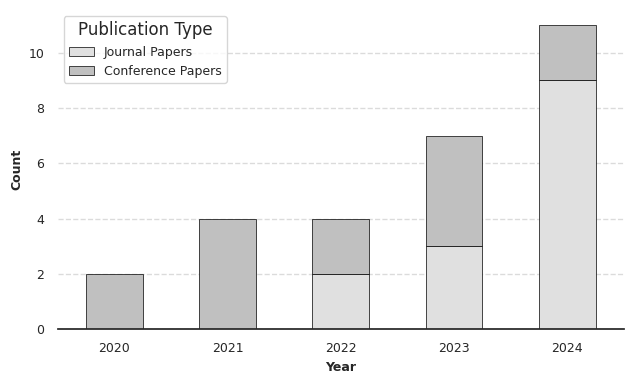
\includegraphics[width=\textwidth]{figs/research_results/publications-stats.png}
        \caption[Publication distribution (2020-2024)]{Distribution of selected publications per year and publication type.}
        \label{fig:publication-stats}
    \end{subfigure}
    \hfill 
    \begin{subfigure}{0.49\textwidth}
        \centering
        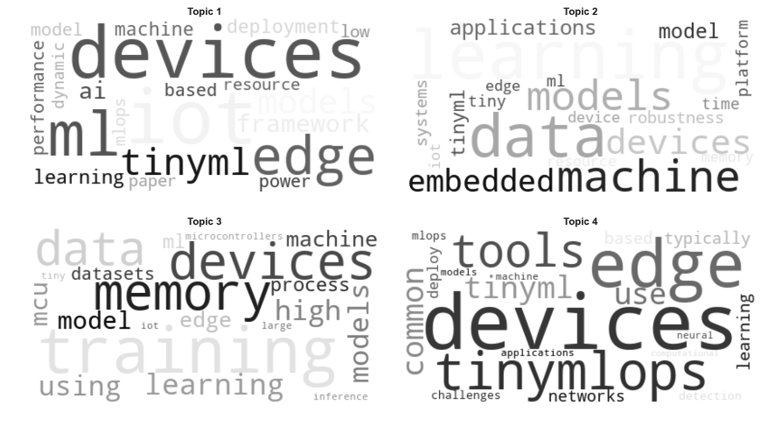
\includegraphics[width=\textwidth]{figs/research_results/topic_modelling.png}
        \caption[Topic modeling of research abstracts]{Topic modeling results from abstracts of the 28 selected papers.}
        \label{fig:TopicModelling}
    \end{subfigure}
    \caption{Temporal and thematic analysis of \gls{tinymlops} research.}
    \label{fig:combined-figures}
\end{figure}

Applying topic modeling to the study abstracts provided deeper insight into thematic patterns, revealing four distinct research clusters (visualized in Figure~\ref{fig:TopicModelling}). The first cluster, Topic 1, centers on the implementation challenges of \gls{ml} deployment on edge devices. Keywords like ``devices'', ``edge'', ``\gls{tinyml}'', and ``perfromance'' highlight resource and energy considerations in \gls{tinyml} applications. In contrast, Topic 2 emphasizes data management within embedded and \gls{iot} environments. This focus is evidenced by the prominence of terms such as ``data'', ``embedded'', ``models'', and ``device'', indicating an emphasis on data-driven adaptation strategies.
The third cluster, Topic 3, addresses the technical constraints of memory utilization and training procedures for \gls{mcu}-based systems. Here, the prevalence of keywords like ``memory'', ``training'', ``model'', and ``\gls{mcu}'' reflects the challenge of executing resource-intensive training operations within severe memory limitations. Finally, Topic 4 concentrates on tooling infrastructure and integrated \gls{mlops} methodologies. Terms including ``tools'', ``\gls{tinymlops}'', ``edge'', and ``device'' signify an emerging focus on comprehensive workflow solutions that address the complexity of model \gls{lcm} in edge computing contexts.

\section{Quantitative Findings from Primary Studies}
\label{sec:QuantitativeFindingsResults}

This section presents a quantitative analysis of the primary studies, examining several dimensions that characterize current \gls{tinymlops} research based on the data extraction framework from Section~\ref{sec:LiteratureReviewProcess}. The analysis proceeds by first exploring research and contribution types (Section~\ref{ssec:ResearchContributionTypeResults}), followed by hardware platforms (Section~\ref{ssec:HardwarePlatformsResults}), \gls{ai} use cases (Section~\ref{ssec:AIUseCaseResults}), system architectures (Section~\ref{ssec:SystemArchitectureResults}), and finally, model training and \gls{lcm} (Section~\ref{ssec:TrainingManagementResults}).

\subsection{Research and Contribution Type}
\label{ssec:ResearchContributionTypeResults}

Following the data synthesis methodology (Section~\ref{subsec:DataSynthesis}), this work classified each publication according to two orthogonal dimensions: research type and contribution type. Research types were categorized using the taxonomy from Wieringa et al. \cite{wieringaRequirementsEngineeringPaper2006}, which distinguishes between solution proposals, validation research, evaluation research, philosophical papers, and experience reports.

\begin{figure}[htbp]
    \centering
    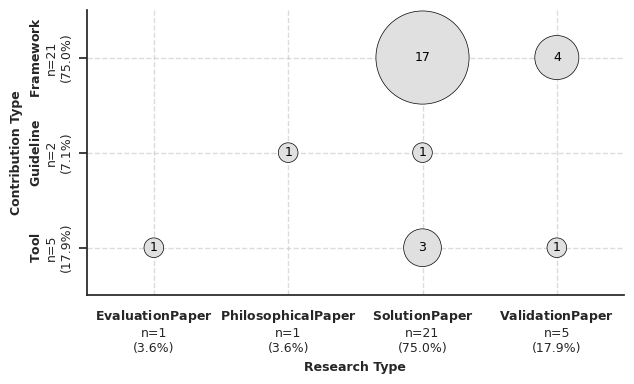
\includegraphics[width=0.8\textwidth]{figs/research_results/contribution-research-type.png}
    \caption[Research and Contribution Type Distribution]{Distribution of \gls{tinymlops} publications by research and contribution type.}
    \label{fig:ResearchContribution}
\end{figure}

Figure~\ref{fig:ResearchContribution} visualizes the distribution of these classifications. The diagram shows 17 publications (approx. 61\%) are solution proposals introducing frameworks, indicating most current research conceptualizes architectural approaches or methodological frameworks for \gls{tinymlops}. Such a focus aligns with the field's nascent state, where researchers establish foundational frameworks to address challenges from resource-constrained environments. In contrast, the lower number of validation studies ($n=5$, approx. 18\%) and evaluation studies ($n=1$, approx. 4\%) suggests a gap in the empirical assessment of proposed solutions. Similarly, the limited presence of guidelines ($n=2$, approx. 7\%) and tooling contributions ($n=5$, approx. 18\%) indicates that the field may not yet have reached a maturity level where comprehensive guidance and standardized toolchains are widely established. This observation aligns with the findings of Kreuzberger et al. \cite{kreuzbergerMachineLearningOperations2023}, who identified similar patterns in the broader \gls{mlops} domain. It suggests that \gls{tinymlops} follows comparable evolutionary trajectories, albeit at an earlier stage of development.
The prevalence of conceptual frameworks ($n=21$, 75\%) coupled with the relative scarcity of empirical validation underscores an imbalance in the current research landscape. More comprehensive real-world validations and longitudinal studies are therefore needed to substantiate the efficacy of proposed \gls{tinymlops} frameworks in production environments.

\subsection{Hardware Platforms and Runtime Environments}
\label{ssec:HardwarePlatformsResults}

Unlike previous reviews with unstructured hardware listings \cite{capogrossoMachineLearningOrientedSurvey2024, rayReviewTinyMLStateoftheart2022, tekinReviewOndeviceMachine2024}, this thesis categorizes platforms based on computational capacity, memory constraints, and operational environment. This classification scheme, presented in Table~\ref{tab:hardware-classification}, distinguishes four primary categories: Ultra-Low-Power, Mid-Range, High-Performance, and \glspl{sbc}.\footnote{The four hardware classes were derived in an iterative session with the OpenAI \textit{ChatGPT} model o1, complemented by targeted web searches (data-sheet specifications and vendor documentation) to anchor the final thresholds in publicly available sources.}

\begin{table}[htbp]
    \caption[Hardware Classification for TinyML Systems]{Hardware Classification for \gls{tinyml} Systems.}
    \label{tab:hardware-classification}
    \begin{tabularx}{\linewidth}{@{}lX@{}}
        \toprule
        \hl{Category}          & \hl{Description} \\
        \midrule
        Ultra-Low-Power        & Clock speed typically below \SI{100}{\mega\hertz}; RAM from a few \gls{kb} to low three-digit \gls{kb} range. \\
        Mid-Range              & Clock speed typically \SIrange{80}{150}{\mega\hertz}; RAM from \SI{32}{\kilo\byte} to \SI{512}{\kilo\byte}. \\
        High-Performance       & Clock speed from approx. \SI{120}{\mega\hertz} to over \SI{600}{\mega\hertz}; RAM from several hundred \gls{kb} up to \SIrange{1}{2}{\mega\byte} on-chip (possibly with additional PSRAM). \\
        Single-Board Computers & Processors such as ARM Cortex-A or similar; run a full OS (e.g., Linux); RAM typically \SI{512}{\mega\byte} or more, often several \gls{gb}. \\
        \bottomrule
    \end{tabularx}
\end{table}

The distribution of hardware platforms across the reviewed literature is depicted in Figure~\ref{fig:hardware-platforms}. High-Performance boards predominate, featured in a majority of studies. This preference suggests that researchers often select devices with sufficient computational capacity for more complex inference tasks, while still aiming for energy efficiency advantages over conventional computing platforms \cite{tekinReviewOndeviceMachine2024}. The second most represented category comprises Mid-Range hardware, which balances computational capability and energy conservation, typically supporting optimized but constrained \gls{ml} models \cite{davidTensorFlowLiteMicro2021}. \Glspl{sbc} constitute a moderate proportion of the studied platforms; implementations frequently leverage multi-process capabilities of conventional operating systems or specialized hardware accelerators (e.g., TPUs, GPUs) \cite{tekinReviewOndeviceMachine2024}. In contrast, Ultra-Low-Power devices receive comparatively limited attention, reflecting the trade-off between minimal energy consumption and computational feasibility for \gls{ml} workloads.

Among specific hardware implementations, the Raspberry Pi 4 Model 4B and the Arduino Nano 33 BLE each appear in five studies (approx. 18\%), while the nRF52840 board is featured in four publications (approx. 14\%). This concentration may indicate the emergence of de facto standard platforms for \gls{tinyml} research and development.
Complementing the hardware analysis, Figure~\ref{fig:runtime-env} illustrates the distribution of runtime environments. Approximately half of the reviewed implementations ($n=15$, approx. 54\%) utilize compiled runtimes to maximize performance. While such approaches optimize execution latency for inference, they can introduce complexity for frequent model updates \cite{banburyEdgeImpulseMLOps2023}. This trade-off becomes critical in production environments where model evolution necessitates streamlined update mechanisms \cite{lootusVMContainerizedApproach2022}. Interpreter-based environments ($n=12$, approx. 43\%) predominantly employ MicroPython implementations. Despite generally lower performance, these environments offer flexibility through lightweight bytecode execution and specialized numerical libraries \cite{antoniniTinyMLOpsFrameworkOrchestrating2022}. The limited representation of \gls{onnx}-based runtimes ($n=2$, approx. 7\%) suggests that vendor-specific inference engines continue to dominate the \gls{tinyml} landscape. Broader adoption of standardized interchange formats like \gls{onnx} could enhance model portability and deployment flexibility, albeit potentially requiring adaptations to existing toolchains \cite{fraidlingTinyMachineLearning2023}.

\begin{figure}[htbp]
    \centering
    \begin{subfigure}{0.64\textwidth}
        \centering
        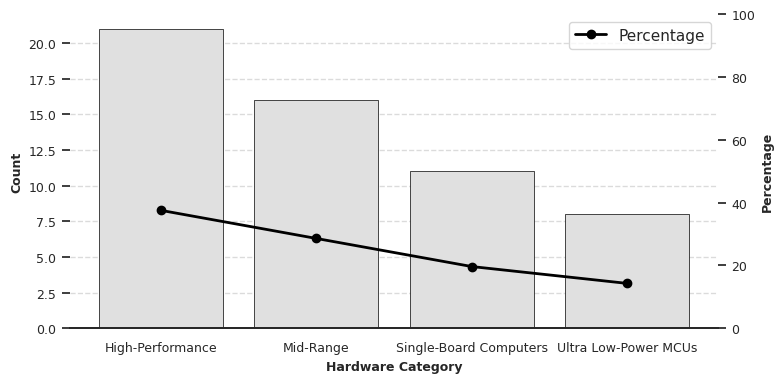
\includegraphics[width=\textwidth]{figs/research_results/hardware-platforms.png}
        \caption[Hardware platform distribution]{Distribution of hardware platforms in reviewed studies.}
        \label{fig:hardware-platforms}
    \end{subfigure}
    \hfill
    \begin{subfigure}{0.34\textwidth}
        \centering
        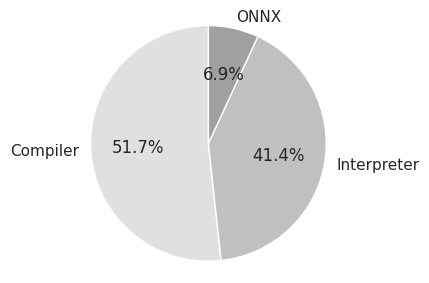
\includegraphics[width=\textwidth]{figs/research_results/runtime.png}
        \caption[Runtime environment distribution]{Runtime environment usage in reviewed studies.}
        \label{fig:runtime-env}
    \end{subfigure}
    \caption{Hardware platforms and runtime environments in \gls{tinymlops} implementations.}
    \label{fig:hardware-vs-runtime}
\end{figure}

\subsection{AI Use Cases and Data Modalities}
\label{ssec:AIUseCaseResults}

To identify primary application domains, the literature corpus was analyzed according to \gls{ai} tasks and corresponding input data modalities. Figure~\ref{fig:ai-use-cases} summarizes the principal \gls{ai} domains. Computer Vision applications constitute one-third of documented use cases (33\%, $n \approx 9$)\footnote{Percentages for AI use cases and data types are based on counts of application instances, where a single paper may report multiple use cases or data types, leading to adjusted counts if summed directly from $N=28$ papers. The text reports proportions based on the total number of identified instances.}, encompassing tasks such as object detection, classification, and segmentation (e.g., \cite{azevedoDetectingFaceMasks2023a}, a face mask detection system on ultra-low-power \glspl{mcu}). Audio Processing represents approximately 20\% of implementations ($n \approx 5$), with keyword spotting and acoustic scene analysis being prevalent (e.g., \cite{grauOnDeviceTrainingMachine2021}). Sensor-based Analysis is the largest category, comprising nearly half of use cases (47\%, $n \approx 13$), and includes diverse applications like anomaly detection, time-series forecasting, and environmental monitoring (e.g., an industrial anomaly detection system \cite{antoniniTinyMLOpsFrameworkOrchestrating2022}). For a more granular understanding, Appendix~\ref{app:detailed-ai-use-cases} provides a detailed breakdown of specific use cases via Figure~\ref{fig:detailed-ai-use-cases}.

\begin{figure}[htbp]
    \centering
    \begin{subfigure}{0.49\textwidth}
        \centering
        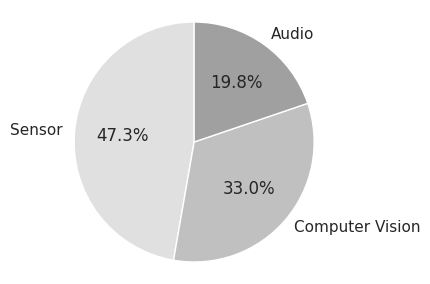
\includegraphics[width=\textwidth]{figs/research_results/sms_used_ai_type.png}
        \caption[AI use case distribution]{Distribution of AI use cases.}
        \label{fig:ai-use-cases}
    \end{subfigure}
    \hfill
    \begin{subfigure}{0.49\textwidth}
        \centering
        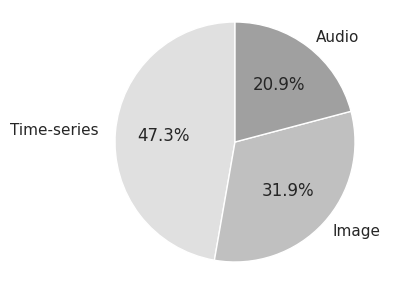
\includegraphics[width=\textwidth]{figs/research_results/sms_used_input_data_type.png}
        \caption[Input data type distribution]{Distribution of input data types.}
        \label{fig:input-data}
    \end{subfigure}
    \caption{AI applications and input data types in \gls{tinymlops} research.}
    \label{fig:ai-use-case-vs-input}
\end{figure}

The distribution of input data types, illustrated in Figure~\ref{fig:input-data}, corroborates the application domain analysis. Time-series data represents nearly half of the studied implementations (47\%, $n \approx 13$), aligning with the prevalence of sensor-driven analytics. Image data accounts for approximately one-third of cases (32\%, $n \approx 9$), corresponding to vision-oriented applications. Audio data completes the distribution at roughly 21\% ($n \approx 6$), reflecting the deployment of on-device speech recognition and acoustic analysis systems.

This categorization of \gls{ai} use cases provides context for addressing RQ3 (from Section~\ref{sec:ResearchObjectivesAndQuestions}). The predominance of sensor-based applications suggests that \gls{tinymlops} frameworks should prioritize efficient processing of time-series data and accommodate operational patterns of continuous sensor monitoring.

\subsection{System Architecture Patterns}
\label{ssec:SystemArchitectureResults}

Figure~\ref{fig:sysAarch} demonstrates the distribution of system architecture patterns that the surveyed articles present. Although the \gls{tinymlops} paradigm inherits many established \gls{devops} and \gls{mlops} workflows, it typically requires specialized optimizations for resource-constrained deployments.

\begin{figure}[htbp]
    \centering
    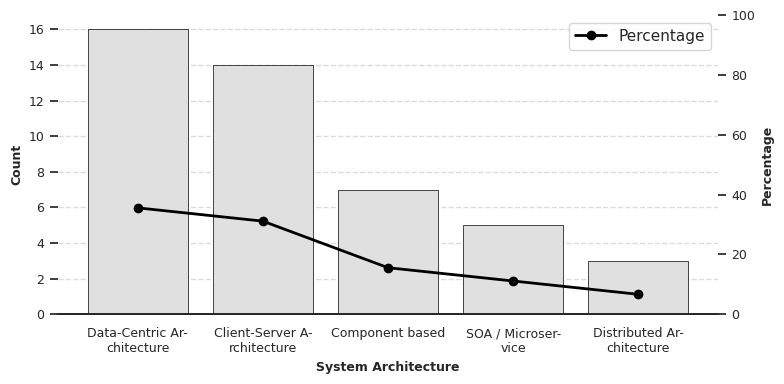
\includegraphics[width=0.975\textwidth]{figs/research_results/sms-system-architecture.png}
    \caption[Distribution of system architecture patterns]{Distribution of system architecture patterns in \gls{tinymlops} literature.}
    \label{fig:sysAarch}
\end{figure}

Data-Centric Architectures lead with a 36\% share ($n=16$ of 45 architectural instances counted across papers)\footnote{Architectural pattern counts may exceed the number of papers (28) as some studies discuss or implement multiple architectures.}, emphasizing refined data pipelines for preprocessing, retraining, and incremental updates \cite{rajEdgeMLOpsAutomation2021, leTinyMLOpsRealtimeUltralow2023a}. Client-Server Architectures follow at 31\% ($n=14$), indicating that numerous \gls{tinyml} solutions remain partially reliant on cloud-based resources \cite{minSensiXBringingMLOps2023, fraidlingTinyMachineLearning2023}. Furthermore, 16\% of instances ($n=7$) implement Component-Based approaches that encapsulate independent functionalities for more agile updates. In contrast, only 11\% ($n=5$) rely on SOA/Microservices, possibly due to overheads from microservice decomposition on highly resource-constrained devices. Distributed Architectures occur in a minimal 7\% of instances ($n=3$), often in the context of  \gls{fl}, which was not a primary focus in most reviewed studies and thus appears underrepresented. Consequently, \gls{tinyml} architectures frequently adapt high-level \gls{mlops} principles—particularly data processing flows—to device-limited contexts. As pragmatic choices, these architectures predominantly use data-centric or hybrid cloud-edge topologies.

\subsection{Model Training and Lifecycle Management}
\label{ssec:TrainingManagementResults}

Addressing model adaptability and \gls{lcm} is pivotal in \gls{tinymlops}. Figure~\ref{fig:training-learning-vs-lcm} illustrates key findings regarding model training approaches (Figure~\ref{fig:training-learning}) and the extent to which studies address \gls{lcm} (Figure~\ref{fig:lcm-done}).

Model Training was classified into three categories based on the location and dependency of the training process \cite{capogrossoMachineLearningOrientedSurvey2024}:

\begin{itemize}[noitemsep, topsep=0pt]
    \item \textit{Central Training}: The \gls{ml} model is trained primarily in a cloud or centralized infrastructure. This method involves data transfer from edge devices to a central server, followed by deployment of the trained model to edge devices.
    \item \textit{Decentral Training}: Training occurs directly on the edge device, without primary reliance on cloud infrastructure. This enables on-device learning and adaptation to local data while reducing cloud dependencies.
    \item \textit{Hybrid Training}: Combines central and decentralized training approaches. This may involve initial training in a central environment, followed by on-device fine-tuning or incremental updates.
\end{itemize}

Model Learning Type was categorized based on the model's adaptation behavior during operation:
\begin{itemize}[noitemsep, topsep=0pt]
    \item \textit{Offline Learning}: The model is trained as a static entity before deployment. No further updates occur during operation \cite{capogrossoMachineLearningOrientedSurvey2024}.
    \item \textit{Online Learning}: The model continuously updates during operation, adapting to newly encountered data \cite{renOndeviceOnlineLearning2024}.
    \item \textit{Incremental Learning}: The model undergoes periodic updates, improving based on new but limited datasets while maintaining prior knowledge \cite{disabatoIncrementalOnDeviceTiny2020}.
\end{itemize}

\begin{figure}[htbp]
    \centering
    \begin{subfigure}{0.62\textwidth}
        \centering
        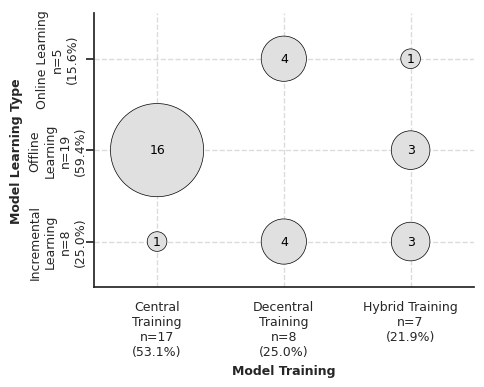
\includegraphics[width=\textwidth]{figs/research_results/sms-training-ort.png}
        \caption[Model training vs. learning type]{Cross-tabulation of training location with learning type.}
        \label{fig:training-learning}
    \end{subfigure}
    \hfill 
    \begin{subfigure}{0.36\textwidth}
        \centering
        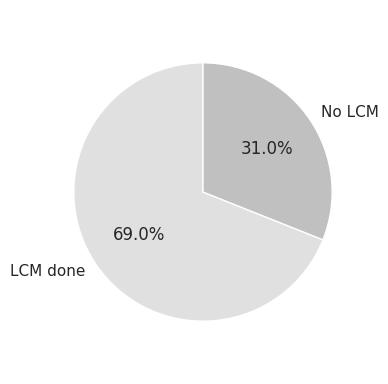
\includegraphics[width=\textwidth]{figs/research_results/lcm-done.png}
        \caption[LCM application in studies]{Share of studies addressing \gls{lcm} practices.}
        \label{fig:lcm-done}
    \end{subfigure}
    \caption{Training approaches and lifecycle management in \gls{tinymlops}.}
    \label{fig:training-learning-vs-lcm}
\end{figure}

Figure~\ref{fig:training-learning} suggests that over half of the examined studies ($n=17$, approx. 53\%) employ Central Training. Nearly all of these ($n=16$) are paired with Offline Learning, indicating a strong preference for pre-trained, static models deployed to edge devices. Although Decentralized Training represents about a quarter of approaches ($n=8$, approx. 25\%), such efforts often emphasize Online Learning ($n=4$) or Incremental Learning ($n=4$), catering to scenarios where on-device model adaptation is essential. Hybrid Training ($n=7$, approx. 22\%) introduces transitional solutions, such as training large base models in the cloud and then fine-tuning or updating incrementally on edge devices. However, given the relatively small number of hybrid-training papers, further validation of these techniques is warranted.

Likewise, Figure~\ref{fig:lcm-done} shows that approximately 69\% of studies ($n=19$) address \gls{lcm}. These articles discuss long-term performance monitoring, redeployment strategies, versioning systems for embedded models, and other operational considerations vital for reliability \cite{huangRIOTMLToolkitOvertheair2024a, sudharsanOTATinyMLAirDeployment2022}. Nonetheless, about 31\% of studies ($n=9$) do not cover \gls{lcm} at all. This potentially leaves open questions regarding safe and resilient continuous deployment for \gls{tinyml} systems across their entire operational lifecycle.

Overall, these findings indicate a continued tendency toward statically trained models for small edge devices. Yet, the potential for real-time or local adaptation in \gls{tinyml} is fostering research on more dynamic training paradigms and a clearer emphasis on the entire lifecycle, bridging initial development, deployment, and ongoing maintenance.

\section{Mapping Studies of Interdependencies}
\label{sec:MappingStudiesResults}

To further elucidate interdependencies within the \gls{tinymlops} landscape, this section builds upon the preceding findings by presenting detailed cross-tabulation analyses. These multi-dimensional mappings explore relationships between aspects such as system architecture, hardware, model training (Section~\ref{ssec:ArchitectureHardwareTrainingResults}), management practices (Section~\ref{ssec:ArchitectureTrainingManagementResults}, Section~\ref{ssec:ManagementLearningMonitoringResults}), CI/CD tactics with optimization techniques (Section~\ref{ssec:CICDTrainingOptimizationResults}), and finally, hardware platforms with \gls{ai} use cases (Section~\ref{ssec:HardwareAIUseCasesResults}). The goal is to reveal complex patterns not apparent from single-dimension analyses, offering deeper insights into current research configurations.

\subsection{Interplay of Architecture, Hardware, and Model Training}
\label{ssec:ArchitectureHardwareTrainingResults}

Figure~\ref{fig:bubble-chart-arch-hw-training} illustrates the distribution of studies across these three dimensions, with bubble size representing frequency. Hardware platforms follow the taxonomy from Table~\ref{tab:hardware-classification}, while system architectures and model training approaches correspond to classifications in Sections~\ref{ssec:SystemArchitectureResults} and \ref{ssec:TrainingManagementResults}.

\begin{figure}[htbp]
    \centering
    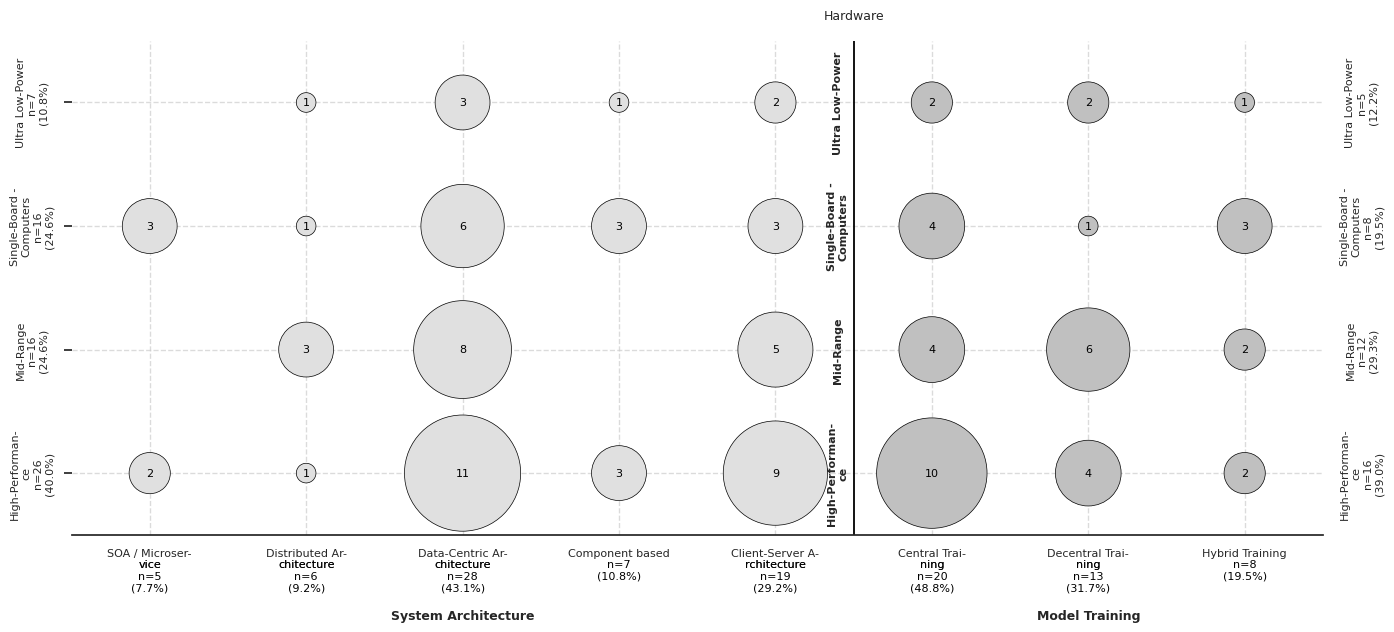
\includegraphics[width=1\textwidth]{figs/research_results/sms_archi-training-hardware.png}
    \caption[Mapping of System Architecture, Hardware, and Training]{Relationship between system architecture, hardware platform, and model training in \gls{tinymlops} implementations.}
    \label{fig:bubble-chart-arch-hw-training}
\end{figure}

Analyzing System Architecture and Hardware Platform dimensions reveals distinct pairing preferences. Data-Centric Architectures are predominant in High-Performance ($n=11$) and Mid-Range Hardware ($n=8$) implementations, appearing less frequently in \glspl{sbc} ($n=6$) and Ultra-Low-Power Hardware ($n=3$). This distribution suggests data-centric approaches are viable across the hardware spectrum but gravitate towards more capable platforms, likely reflecting computational demands of comprehensive data processing.
Similarly, Client-Server architectures appear most frequently with High-Performance ($n=9$) and Mid-Range Hardware ($n=5$), with modest representation in \glspl{sbc} ($n=3$) and Ultra-Low-Power boards ($n=2$).
Conversely, Distributed Architectures concentrate primarily in Mid-Range ($n=3$) and Ultra-Low-Power ($n=1$ instance) categories, with minimal representation in high-performance contexts. This pattern reflects the specialized nature of distributed architectures within \gls{tinymlops}, often tied to \gls{fl} implementations \cite{grauOnDeviceTrainingMachine2021}. The limited overall presence of distributed approaches stems from the study's scope rather than indicating irrelevance to the broader field.\footnote{The discrepancy in Distributed Architecture counts compared to Section~\ref{ssec:SystemArchitectureResults} arises because individual studies often evaluate multiple hardware configurations while maintaining a consistent architectural approach.}
SOA/Microservices approaches manifest infrequently overall. When employed, they cluster with High-Performance Hardware ($n=2$) and \glspl{sbc} ($n=3$), with no presence in Mid-Range or Ultra-Low-Power categories. This distribution suggests the inherent overhead of microservice architectures restricts their deployment to edge devices with substantial computational resources \cite{rajEdgeMLOpsAutomation2021}. A comparable distribution characterizes Component-Based Architectures, appearing relatively evenly across High-Performance Hardware ($n=3$) and \glspl{sbc} ($n=3$), but diminishing considerably in mid-range and ultra-low-power categories

Regarding the relationship between hardware platforms and training methodologies, Central Training approaches cluster predominantly with High-Performance ($n=10$), Mid-Range ($n=4$), and \glspl{sbc} ($n=4$). This confirms a trend of cloud-based training being common across various capable hardware categories.
In contrast, Decentralized Training strategies are more distributed, appearing most with Mid-Range hardware ($n=6$), followed by High-Performance ($n=4$), with fewer implementations in Ultra-Low-Power ($n=2$) and \glspl{sbc} ($n=1$). This pattern indicates on-device training is gaining traction even in moderately constrained environments.
Hybrid Training configurations span diverse hardware, with a relative concentration in \gls{sbc} implementations ($n=3$ studies) and High-Performance ($n=2$). This suggests hybrid approaches may balance edge autonomy with computational feasibility, such as solutions leveraging pre-trained feature extractors with locally adaptable classification layers \cite{disabatoIncrementalOnDeviceTiny2020}.

Cross-referencing these analyses unveils a significant cluster around Client-Server and Data-Centric Architectures on High-Performance boards using Central Training. This recurring pattern signals a preference for these architectures on capable edge platforms while offloading intensive training to cloud infrastructure (e.g., \cite{banburyEdgeImpulseMLOps2023}). Furthermore, this configuration underscores the relationship between client-server architectures and cloud services beyond model training, as demonstrated in frameworks for collaborative inference \cite{antoniniTinyMLOpsFrameworkOrchestrating2022}. Broader findings also indicate that while ultra-low-power implementations exist, their integration within dominant high-performance paradigms remains sparse, suggesting relevance primarily in specialized applications prioritizing extreme energy efficiency \cite{pavanTyBoxAutomaticDesign2024}.
Overall, the mapping reveals that while central training is predominant, training methodology selection is not strictly determined by hardware tier. It reflects a complex interplay of factors, including the ongoing exploration of decentralized and hybrid approaches across the \gls{tinymlops} spectrum.

\subsection{Interplay of Architecture, Training, and Model Management}
\label{ssec:ArchitectureTrainingManagementResults}

Expanding on the hardware-centric analysis (Section~\ref{ssec:ArchitectureHardwareTrainingResults}), this subsection incorporates Model Management practices for a more comprehensive perspective on operational patterns. Figure~\ref{fig:bubble-chart-arch-training-mgmt} visualizes the distribution of primary studies across System Architecture, Model Training methodologies, and Model Management practices.

\begin{figure}[htbp]
    \centering
    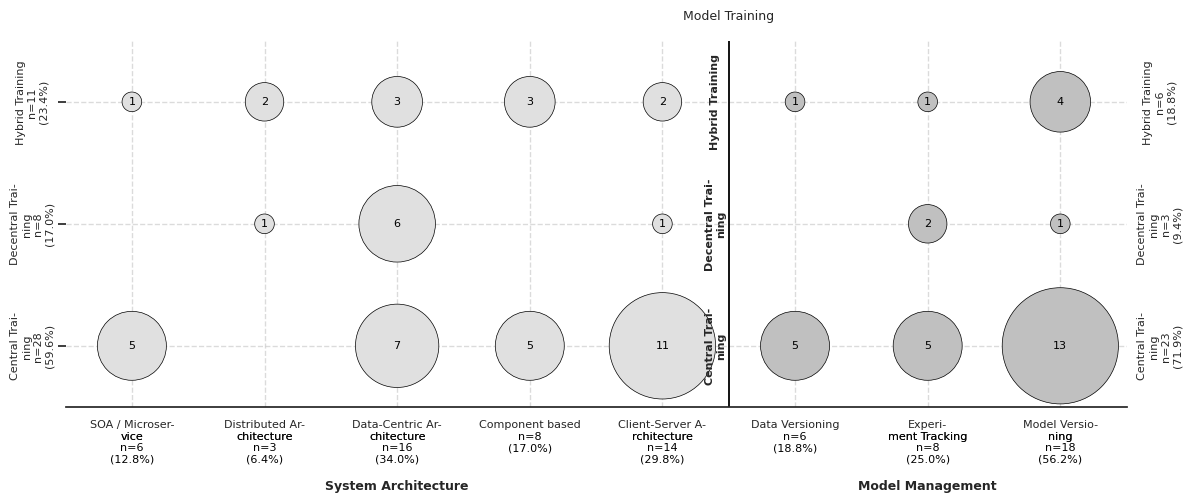
\includegraphics[width=1\textwidth]{figs/research_results/sms_archi-training-lcm.png}
    \caption[Mapping of System Architecture, Training, and Management]{Correlation between system architecture, model training, and model management practices.}
    \label{fig:bubble-chart-arch-training-mgmt}
\end{figure}

Mapped relationships confirm that SOA/Microservices and Distributed Architectures, consistent with their limited overall presence (Section~\ref{ssec:ArchitectureHardwareTrainingResults}), show minimal representation across management and training combinations. Proportionally, SOA/Microservices architectures show an almost exclusive affinity with Central Training ($n=5$). A similar pattern emerges for Component-Based architectures ($n=5$ with Central Training, $n=3$ with Hybrid). These correspondences suggest implementing microservice-based and component-based architectures often involves cloud infrastructure for model training. Such configurations typically occur within larger, complex systems where cloud integration and sophisticated tooling are prevalent \cite{fraidlingTinyMachineLearning2023}. This aligns with Section~\ref{ssec:ArchitectureHardwareTrainingResults}, where both architectural approaches appeared less frequently, likely due to resource demands in constrained environments.
Distributed Architectures show sparse representation, particularly with hybrid and decentralized training. This aligns with \gls{fl} principles, where models train on edge devices, with only weight updates transmitted centrally.
Data-Centric Architectures, while prevalent across all training methodologies, display a modest concentration with Central Training ($n=7$) alongside considerable presence with Decentral Training ($n=6$). This balance underscores the versatility of data-centric approaches for diverse training paradigms, from cloud-based batch learning to adaptive on-device techniques.
In contrast, Client-Server Architectures demonstrate a pronounced preference for Central Training ($n=11$), reinforcing their reliance on robust, centralized training infrastructure—a pattern consistent with hardware associations in Section~\ref{ssec:ArchitectureHardwareTrainingResults}.

Shifting focus to Model Management techniques and their relationship with training methodologies reveals additional patterns. Within the corpus, Model Management practices include Data Versioning ($n=6$, approx. 19\%), Experiment Tracking ($n=8$, approx. 25\%), and Model Versioning ($n=18$, approx. 56\%). Among these, Model Versioning is the predominant practice across all training approaches, with particular dominance alongside Central Training ($n=13$). This strong association reflects the established \gls{mlops} emphasis on rigorous model version control in centralized development.
Experiment Tracking similarly gravitates toward Central Training ($n=5$) but also appears with decentralized ($n=2$) and hybrid ($n=1$) approaches, suggesting broader applicability. Notably, while model versioning predominates overall, experiment tracking appears proportionally more frequent in decentralized contexts.\footnote{One might postulate that Experiment Tracking and Model Versioning are typically employed in tandem, particularly in Decentral Training. However, this does not appear to be the case within reviewed studies. This observation might stem from \gls{fl} emphasis on transmitting model weights rather than explicit versioning. Definitive confirmation requires additional research given the limited number of \gls{fl} papers in this study.}
Data Versioning, though less common, also concentrates primarily with Central Training ($n=5$). This suggests robust data management practices feature predominantly in centralized \gls{tinyml} pipelines, aligned with established data-centric \gls{mlops} workflows.

Collectively, these mappings highlight that Central Training not only remains the prevailing paradigm in \gls{tinymlops} but also shows substantial integration with established \gls{mlops} practices like Model Versioning and Experiment Tracking. The convergence of Client-Server Architecture, Central Training, and Model Versioning represents a predominant configuration: leveraging client-server topologies with cloud-based training while implementing rigorous model version control. This reinforces the pattern from Section~\ref{ssec:ArchitectureHardwareTrainingResults}, where client-server architectures frequently paired with high-performance hardware and central training, indicating a consistent architectural approach.
Nevertheless, the emerging presence of Decentral Training and Hybrid Training alongside Experiment Tracking signals an incipient shift toward more agile, on-device \gls{mlops} practices, though still in early developmental stages. This nascent trend, while not yet predominant, potentially represents an evolving research direction addressing centralized training limitations in increasingly autonomous edge scenarios.

\subsection{Interplay of Management, Learning, and Monitoring}
\label{ssec:ManagementLearningMonitoringResults}

Deepening the dimensional analysis, this subsection investigates interrelationships between Model Management practices, Model Learning types, and Monitoring metrics. This offers granular insights into \gls{tinymlops} operational dynamics. Figure~\ref{fig:bubble-chart-mgmt-learning-monitoring} visualizes the distribution of primary studies across these dimensions, complementing preceding analyses of architecture, hardware, and training.

The analysis first considers the relationship between Model Management techniques and Model Learning Types. Model Management practices comprise Model Versioning ($n=21$, approx. 57\%), Experiment Tracking ($n=10$, approx. 27\%), and Data Versioning ($n=6$, approx. 16\%). Monitoring metrics include Model Accuracy ($n=23$, approx. 33\%), Concept/Data Drift ($n=19$, approx. 27\%), Computational Latency ($n=18$, approx. 26\%), and RAM Usage ($n=10$, approx. 14\%). Consistent with patterns in Section~\ref{ssec:TrainingManagementResults}, Offline Learning predominates, followed by Incremental Learning and Online Learning.

\begin{figure}[htbp]
    \centering
    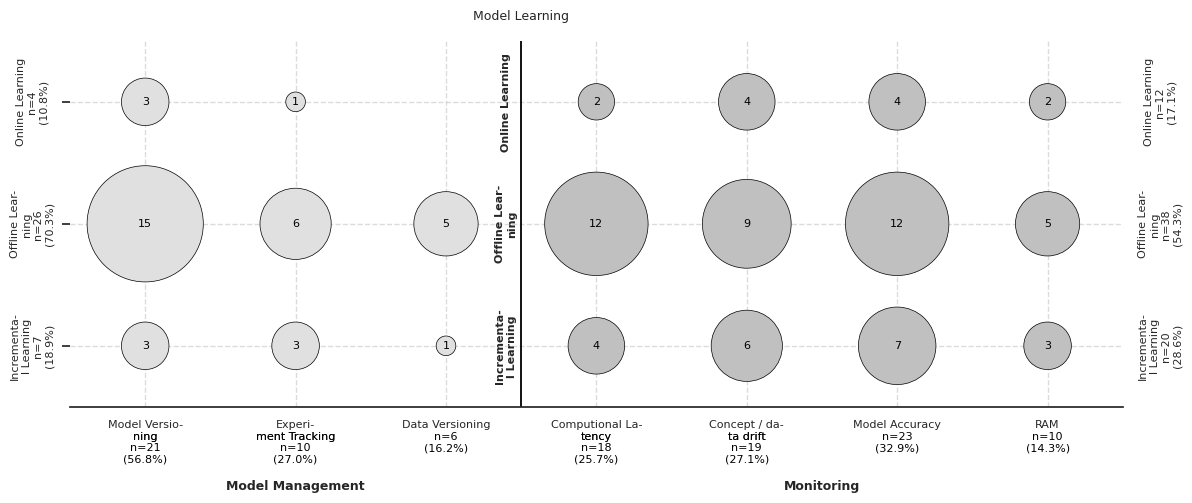
\includegraphics[width=1\textwidth]{figs/research_results/sms-learning-monitoring.png}
    \caption[Mapping of Model Management, Learning, and Monitoring]{Integration of model management, learning types, and monitoring metrics in \gls{tinymlops} systems.}
    \label{fig:bubble-chart-mgmt-learning-monitoring}
\end{figure}

Examination of mapped relationships reveals that Model Versioning, while prominent across all learning categories, converges markedly with Offline Learning ($n=15$). This pairing reinforces the established \gls{mlops} emphasis on version control for statically trained models, aligning with the broader tendency toward centralized training and offline deployment.
Experiment Tracking, though less frequent, similarly gravitates toward Offline Learning ($n=6$) while maintaining some presence with Incremental Learning ($n=3$) and Online Learning ($n=1$). This pattern suggests experiment tracking's applicability across learning paradigms, though still predominantly in offline contexts.
Data Versioning, the least common management practice, also concentrates primarily with Offline Learning ($n=5$), indicating that explicit data management typically accompanies static, pre-deployment training workflows.

The secondary mapping examines Monitoring Metrics in relation to Model Learning Types. Model Accuracy and Computational Latency monitoring strongly associate with Offline Learning ($n=12$ for both). These dual concentrations highlight practical priorities for offline learning: ensuring high model performance and efficient inference on resource-constrained hardware.
Concept/Data Drift monitoring, while slightly less prevalent, shows notable correlation with Incremental Learning ($n=6$). This association indicates drift detection's relevance for adaptive models undergoing periodic updates that must maintain performance in evolving environments.
RAM Usage, the least common monitoring metric, distributes relatively uniformly across learning types. This suggests memory consumption is a device-level concern spanning different learning paradigms rather than being specifically emphasized by one approach.

Collectively, these mappings reinforce the overarching pattern that Offline Learning and Central Training remain predominant. They show strong connections to established practices like Model Versioning and a dual focus on Model Accuracy and Computational Latency as primary performance indicators.
Notably, while Experiment Tracking and Data Versioning appear less frequently, their associations with Offline Learning suggest conventional \gls{tinymlops} workflows are beginning to incorporate elements of systematic experimentation and data management. Interestingly, monitoring metrics, when analyzed proportionally to each learning type, distribute relatively evenly across different approaches and management practices. This balanced distribution indicates monitoring is a fundamental aspect of \gls{tinymlops}, regardless of specific learning or management strategy. Whether implementing static, pre-trained models or adaptive, on-device learning, continuous assessment of performance, resource utilization, and phenomena like concept drift remains essential for reliability, efficiency, and operational longevity. This widespread recognition of monitoring's importance may signal the \gls{tinymlops} field's maturation toward more comprehensive operational practices beyond initial model development and deployment, reflecting an increasing emphasis on full \gls{lcm}.

\subsection{Interplay of CI/CD, Training, and Optimization}
\label{ssec:CICDTrainingOptimizationResults}

Building upon previous dimensional analyses, this subsection explores interrelationships between \gls{ci}/\gls{cd} tactics, Model Training methodologies, and Optimization techniques. This provides deeper insights into deployment and efficiency considerations. Figure~\ref{fig:bubble-chart-cicd-training-optimization} visualizes the distribution of primary studies across these dimensions. Detailed descriptions of \gls{ci}/\gls{cd} tactics and optimization techniques can be found in Table~\ref{tab:cicd-optim-techniques} (Appendix).

The mapping first examines \gls{ci}/\gls{cd} Tactics in relation to Model Training types. Within the corpus, \gls{ci}/\gls{cd} tactics comprise Automated Deployment and Full Model Update (both $n=20$, approx. 37\%), followed by Partial Model Update ($n=11$, approx. 20\%) and Automated Tests ($n=3$, approx. 6\%). Optimization Techniques include Quantization and Pruning ($n=17$, approx. 57\%), Test-Time Adaptation and Adaptive Computation (both $n=4$, approx. 13\% each), Feature Caching ($n=3$, 10\%), and Knowledge Distillation ($n=2$, approx. 7\%).

\begin{figure}[htbp]
    \centering
    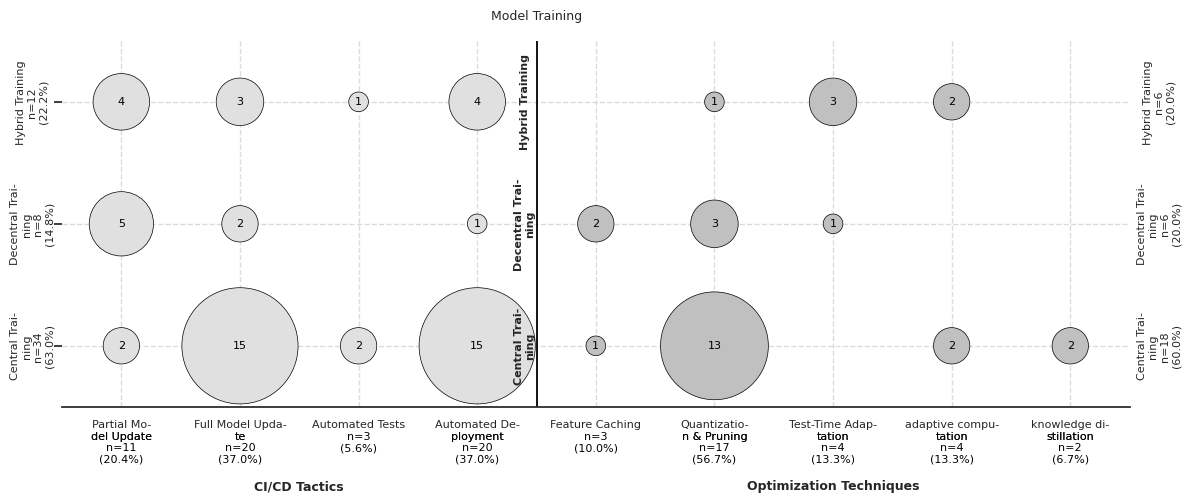
\includegraphics[width=1\textwidth]{figs/research_results/sms_cicd-training-optimization.png} 
    \caption[Mapping of CI/CD Tactics, Training, and Optimization]{CI/CD tactics in relation to model training and optimization techniques.}
    \label{fig:bubble-chart-cicd-training-optimization}
\end{figure}

Analysis of mapped relationships reveals a significant convergence of Full Model Update with Central Training ($n=15$). This association indicates the predominant \gls{ci}/\gls{cd} approach involves complete model replacement within centralized training workflows.
In contrast, Partial Model Update displays a more balanced distribution across Decentral Training ($n=5$) and Hybrid Training ($n=4$). This suggests incremental updates feature more prominently in on-device or hybrid learning contexts where efficient adaptation to new data takes precedence over complete retraining.
Automated Deployment, paralleling Full Model Update, shows strong correlation with Central Training ($n=15$), reinforcing reliance on automated deployment pipelines for centrally trained models.
Automated Tests, though infrequently mentioned as a \gls{ci}/\gls{cd} tactic, also primarily associate with Central Training ($n=2$). This indicates automated testing practices, where present, typically integrate into established, cloud-centric \gls{mlops} workflows alongside full model updates.

The secondary mapping examines Optimization Techniques in relation to Model Training types. This analysis reveals a marked predominance of Quantization and Pruning with Central Training ($n=13$). This strong association underscores that these techniques, as cornerstone \gls{tinyml} optimization methods, are widely used to minimize model size and computational requirements for edge deployment.
Feature Caching and Adaptive Computation, though less common, primarily correlate with Decentral Training ($n=2$ for Feature Caching) and Hybrid Training ($n=2$ for Adaptive Computation). This pattern suggests these specialized optimization techniques appear mainly in scenarios prioritizing on-device adaptation and computational efficiency beyond standard offline optimization.
Test-Time Adaptation similarly shows stronger presence with Hybrid Training ($n=3$) compared to central or decentralized approaches. This indicates its relevance for contexts requiring model fine-tuning or adaptation during deployment, particularly in hybrid training paradigms \cite{moskalenkoResilienceawareMLOpsResourceconstrained2023}.
Knowledge Distillation, the least frequent optimization technique here, associates exclusively with Central Training ($n=2$). This suggests that despite its theoretical potential, knowledge distillation currently receives less emphasis compared to more direct optimization methods like quantization and pruning.

Collectively, these mappings reinforce the overarching trend that Central Training predominates in \gls{tinymlops}. This extends to \gls{ci}/\gls{cd} tactics like Full Model Update and Automated Deployment, and fundamental optimization techniques like Quantization and Pruning. This predominance underscores a current emphasis on well-defined, static deployment pipelines, where models undergo central development, optimization, and deployment as complete replacements.
However, the distribution also indicates that while specialized optimization techniques appear less frequently, their emerging associations with Decentral Training and Hybrid Training suggest an incipient trend toward more sophisticated, adaptive optimization strategies in on-device and continuous learning scenarios. This nascent shift, though not yet predominant, potentially represents a research direction aiming to transcend standard compression methods and address the unique efficiency requirements of increasingly autonomous deployments, particularly as exploration of complex on-device learning advances. This observation aligns with the intuition that publications focusing on on-device \gls{mlops} may investigate more advanced technical optimizations beyond conventional \gls{mlops} and \gls{tinyml} workflows \cite{pavanTyBoxAutomaticDesign2024}.

\subsection{Mapping Hardware Platforms to AI Use Cases}
\label{ssec:HardwareAIUseCasesResults}

Departing from study-centric mappings, this subsection adopts a hardware-centric approach to analyze the \gls{tinymlops} deployment landscape. Unlike previous mappings focused on technique prevalence across literature, this analysis directly maps AI Use Cases to specific Hardware Platforms. This shift is crucial as many primary studies evaluate \gls{tinymlops} approaches across multiple hardware platforms or with diverse techniques. For instance, a single study might showcase decentralized incremental training on ultra-low-power devices alongside a client-server architecture using \gls{sbc}s for central retraining and advanced \gls{lcm} \cite{antoniniTinyMLOpsFrameworkOrchestrating2022}. A purely study-centric mapping might not accurately reflect the practical use-case landscape. Therefore, this subsection re-examines dimensions through a hardware-centric lens, building upon the hardware taxonomy (Table~\ref{tab:hardware-classification}) and complementing the use case analysis (Section~\ref{ssec:AIUseCaseResults}).

\begin{figure}[htbp]
    \centering
    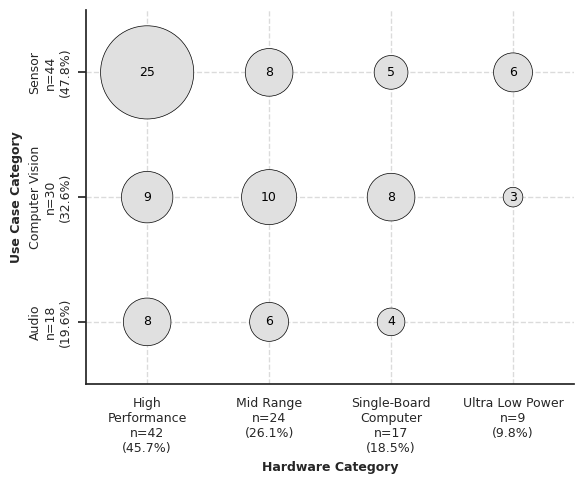
\includegraphics[width=0.8\textwidth]{figs/research_results/sms_hardware_use_case.png} 
    \caption[Mapping of Hardware Platforms to AI Use Cases]{Hardware platform distribution across AI use case categories.}
    \label{fig:bubble-chart-hardware-vs-aiusecase} % Umbenannt für Eindeutigkeit
\end{figure}

Figure~\ref{fig:bubble-chart-hardware-vs-aiusecase} illustrates the relationship between hardware platforms and \gls{ai} use cases. The visualization reveals distinct patterns providing insights into current \gls{tinyml} implementation priorities. For a granular breakdown of specific \gls{ai} applications, refer to Appendix~\ref{app:detailed-ai-use-cases} (Figure~\ref{fig:detailed-ai-use-cases}).

The most prominent pattern is the substantial concentration of High-Performance hardware implementations for Sensor-based applications ($n=25$). This represents the largest single category, suggesting sensor data processing—despite potential assumptions of lower computational needs—currently favors more capable hardware in practice. Examples include \cite{antoniniTinyMLOpsFrameworkOrchestrating2022} (industrial anomaly detection using high-performance \glspl{mcu}) and \cite{fraidlingTinyMachineLearning2023} (sensor data fusion on an STM32-F746NG platform). This may reflect requirements for real-time processing of multiple sensor streams, complex fusion algorithms, or accommodation of continuous on-device learning.

For Computer Vision use cases, closer examination reveals nuances. While Mid-Range hardware shows the highest frequency ($n=10$), these implementations often represent simpler binary classification tasks rather than complex object detection or segmentation. For more advanced computer vision, \glspl{sbc} demonstrate greater prevalence \cite{renOndeviceOnlineLearning2024}. High-Performance platforms ($n=9$) maintain substantial representation across vision tasks, while Ultra-Low-Power devices ($n=3$) show limited adoption, primarily for constrained classification scenarios. Audio processing exhibits a distinct hardware profile: High-Performance platforms ($n=8$) lead, followed by Mid-Range devices ($n=6$) and \glspl{sbc} ($n=4$). As shown in \cite{grauOnDeviceTrainingMachine2021}, keyword spotting is a common audio application on mid-range hardware (e.g., Arduino Nano 33 BLE, Cortex-M4 based platforms). The absence of Ultra-Low-Power devices in audio processing suggests technical barriers for audio-based \gls{tinymlops} on severely constrained hardware, likely due to continuous sampling and spectral processing demands.

\section{System Architectures in TinyML}
\label{sec:RQ1_Results_SystemArchitecture}

Analysis of the selected literature reveals a spectrum of recurring architectural patterns for integrating \gls{tinyml} systems with \gls{mlops} practices, as summarized in Table~\ref{tab:architectural_patterns_overview}. These patterns are not always mutually exclusive; many contemporary \gls{tinyml} systems exhibit hybrid characteristics, borrowing elements from multiple established approaches to achieve desired performance and functionality. Categorized by their primary locus of control and computation—ranging from centralized cloud-dependent models to fully decentralized edge-native solutions—this strategic balancing reflects a growing understanding of harnessing distributed resources effectively for specific application demands and hardware constraints. The subsequent discussion (Sections~\ref{ssec:centralized_hybrid_arch} and \ref{ssec:decentralized_edge_native_arch}) elaborates on these categories, linking them to research contributions and inherent trade-offs.

\begin{landscape}
    \begin{table}[htbp]
        \caption[Overview of System Architecture Patterns]{\emph{Synthesized Overview} of System Architecture Patterns in \gls{tinyml}/\gls{mlops}}
        \label{tab:architectural_patterns_overview}
        \scriptsize
        \renewcommand{\arraystretch}{1.2}
        \setlength{\tabcolsep}{4pt} % Unified tabcolsep
        \begin{tabularx}{\linewidth}{@{} >{\RaggedRight\bfseries\arraybackslash}X % First column now bold by spec
                                     >{\RaggedRight\arraybackslash}X
                                     >{\RaggedRight\arraybackslash}X
                                     >{\RaggedRight\arraybackslash}X
                                     >{\RaggedRight\arraybackslash}X
                                     >{\RaggedRight\arraybackslash}X @{}}
            \toprule
            \hl{\footnotesize\textbf{Architectural Pattern}} &
            \hl{\footnotesize\textbf{Key Components}} &
            \hl{\footnotesize\textbf{Dependencies}} &
            \hl{\footnotesize\textbf{Strengths}} &
            \hl{\footnotesize\textbf{Limitations}} &
            \hl{\footnotesize\textbf{Example (Papers)}} \\
            \midrule
            Data-Centric & 
                Data acquisition, preprocessing modules; Feature extraction, data storage (on-device/edge); Data buffers; on-device/edge learning mechanisms &
                Data availability \& quality; Local processing capacity; Efficient algorithms; Communication for data offloading &
                Optimized data handling; Supports continuous learning \& adaptation to local conditions/drift; Model robustness; Potential for personalization; Reduces data transmission overhead &
                Resource-intensive for complex on-device processing/feature extraction; Relies heavily on data quality at the source; Managing consistency \& quality across devices; Potential for catastrophic forgetting if not managed &
                \cite{banburyEdgeImpulseMLOps2023}, \cite{disabatoIncrementalOnDeviceTiny2020}, \cite{renOndeviceOnlineLearning2024}, \cite{sudharsanEdge2TrainFrameworkTrain2020}, \cite{moskalenkoResilienceawareMLOpsResourceconstrained2023}, \cite{pavanTyBoxAutomaticDesign2024}, \cite{grauOnDeviceTrainingMachine2021}, \cite{fraidlingTinyMachineLearning2023}, \cite{demaghSensOLMemoryEfficientOnline2024} \\
            \midrule
            Client-Server / Edge-Cloud &
                \gls{mcu}/\gls{sbc} as client/edge node; Gateway; Cloud/edge server backend/platform; \gls{ml} tasks split (e.g., inference on device, training in cloud) &
                Network connectivity (may be intermittent); Server availability; Security of data in transit \& at rest; Communication protocols (e.g., \gls{mqtt}, gls{coap}, HTTP, ESP-NOW, \gls{lwm2m}) &
                Powerful cloud/server resources for complex tasks; Simpler/lower-cost edge devices; Centralized management \& \gls{ota} updates; Global model improvements; Edge processing can offer lower latency &
                Dependence on network connectivity and latency; Bandwidth costs/consumption; Privacy concerns with raw data transmission; Complexity in managing distributed components &
                \cite{antoniniTinyMLOpsFrameworkOrchestrating2022}, \cite{fraidlingTinyMachineLearning2023}, \cite{alselekAgileAIFirmware2024}, \cite{alselekDynamicAIIoTEnabling2024}, \cite{rajEdgeMLOpsAutomation2021}, \cite{doyuTinyMLaaSEcosystemMachine2021}, \cite{peltonenLinkEdgeOpensourcedMLOps2023}, \cite{sudharsanOTATinyMLAirDeployment2022}, \cite{zaidiUnlockingEdgeIntelligence2022}, \cite{condeEnhancedFIWAREBasedArchitecture2024}, \cite{huangRIOTMLToolkitOvertheair2024a} \\
            \midrule
            Component-Based &
                Modular software/hardware units (sensing, preprocessing, inference, communication, update agent, etc.) on device and/or server; optional cloud layer &
                Well-defined interfaces; Interface \& version compatibility; Orchestration mechanism &
                Modularity promotes reusability, maintainability, \& independent updates; Simplifies development \& maintenance; agile deployment \& easier replacement of parts &
                Integration complexity between components; Potential overhead from inter-component communication; Requires careful interface design; Resource partitioning challenges &
                \cite{szydloManagementTinyMLEnabled2024}, \cite{sudharsanEdge2TrainFrameworkTrain2020}, \cite{minSensiXBringingMLOps2023}, \cite{pavanTyBoxAutomaticDesign2024}, \cite{lootusVMContainerizedApproach2022}, \cite{fraidlingTinyMachineLearning2023}, \cite{condeEnhancedFIWAREBasedArchitecture2024}, \cite{antoniniTinyMLOpsFrameworkOrchestrating2022}, \cite{rajEdgeMLOpsAutomation2021} \\
            \midrule
            Microservices/\gls{soa} &
                Fine-grained, independent, loosely coupled, deployable services (model serving, data transformation, inference, etc.); APIs for inter-service communication (e.g., \gls{rest} APIs, message queues); Containerized \& managed by orchestrator &
                Network infrastructure; Inter-service communication; Service orchestration; API management, service discovery &
                High scalability \& flexibility; Fault isolation \& resilience; Heterogeneous components/frameworks; Independent development/deployment of services &
                Overhead (memory, compute, network, containerization) for resource-constrained devices; Increased complexity in deployment, management, \& orchestration; Higher latency/network overhead from inter-service calls &
                \cite{minSensiXBringingMLOps2023}, \cite{rajEdgeMLOpsAutomation2021}, \cite{condeEnhancedFIWAREBasedArchitecture2024}, \cite{lootusVMContainerizedApproach2022}, \cite{alselekAgileAIFirmware2024}       \\
            \midrule
            Distributed (Federated/Cooperative) &
                Multiple edge devices capable of local training; Optional central aggregation server (for \gls{fl}) or P2P links; Distributed training/\gls{fl} algorithms (e.g., FedAvg); Communication protocols for model updates/parameters &
                Network connectivity; Standardized model/update formats; Algorithms for model aggregation/consensus; Client participation; Handling stragglers \& data heterogeneity &
                Enhanced privacy (raw data stays local); Leverages knowledge from distributed datasets; Enables collaborative learning; Reduced communication bandwidth (only model updates/parameters shared); Improve model generalization \& robustness &
                Communication overhead for model updates; Complexity of distributed training, orchestration, synchronization; Managing stragglers \& device heterogeneity; Statistical heterogeneity can impede convergence; Security of aggregation process &
                \cite{gulatiTDMiLTinyDistributed2024}, \cite{renOndeviceOnlineLearning2024}, \cite{grauOnDeviceTrainingMachine2021}, \cite{alselekDynamicAIIoTEnabling2024} \\
            \bottomrule
        \end{tabularx}
    \end{table}
\end{landscape}

\subsection{Centralized and Hybrid Architectural Models}
\label{ssec:centralized_hybrid_arch}

A significant portion of \gls{tinyml} systems leverages centralized or hybrid architectural models, where a substantial part of the computational load, control logic, or complex model training resides in a more powerful backend, such as a cloud platform or an edge server. The classic \textit{Client-Server architecture} (often termed \textit{Edge-Cloud} in this context) is a prime example \cite{doyuTinyMLaaSEcosystemMachine2021, zaidiUnlockingEdgeIntelligence2022, peltonenLinkEdgeOpensourcedMLOps2023}. In this setup, resource-constrained \gls{tinyml} devices (clients) primarily handle data acquisition, local preprocessing, and optimized model inference. More demanding tasks—such as initial model training, extensive data processing, complex retraining, model optimization, and overarching \gls{mlops} orchestration including \gls{ci}/\gls{cd} pipelines—are offloaded to the server or cloud components. This division allows \gls{tinyml} devices to overcome their inherent resource limitations by leveraging scalable, centralized resources for storage and computation. Frameworks such as Edge Impulse \cite{banburyEdgeImpulseMLOps2023}, and platforms like Azure IoT Edge, AWS IoT Greengrass, and LinkEdge \cite{peltonenLinkEdgeOpensourcedMLOps2023}, embody this hybrid pattern, often utilizing containerization concepts for deploying and managing \gls{ml} models. The strength of such architectures lies in centralized control, enabling streamlined remote model updates (\gls{ota}), comprehensive monitoring, and adaptation of models. The Edge \gls{mlops} framework by Raj et al.~\cite{rajEdgeMLOpsAutomation2021} further exemplifies this by demonstrating a \gls{ci}/\gls{cd} pipeline that deploys containerized models from a cloud orchestrator to edge devices.

\textit{Component-Based architectures} and \textit{Microservice/\gls{soa} architectures} also frequently manifest within this centralized or hybrid paradigm, particularly when a central orchestrator or cloud backend manages the deployment and interaction of modular components or fine-grained services. For instance, SensiX++ \cite{minSensiXBringingMLOps2023} employs modular components for data coordination and model serving on the edge device, but these are typically part of a larger system where model updates and high-level orchestration are managed centrally. Similarly, microservices deployed on edge gateways might interact with cloud-based services for advanced analytics or model retraining. Components like data coordinators, model servers, and adaptive schedulers often interact within the server/cloud layer to manage the lifecycle of \gls{ml} models destined for the edge. While full microservice deployments are less common directly on severely constrained \glspl{mcu} due to overhead, the principles of modularity and isolated execution are explored, as seen with concepts like ``Runes'' aiming for container-like packages on \glspl{mcu} \cite{lootusVMContainerizedApproach2022}. The emergence of ``as-a-Service'' models, such as \gls{tmlaas} \cite{doyuTinyMLaaSEcosystemMachine2021}, explicitly embodies this hybrid approach, offering \gls{ml} capabilities to constrained devices through services hosted at the edge or in the cloud. The primary advantages include leveraging powerful centralized resources and maintaining a unified control plane. However, these models inherently depend on reliable network connectivity, and data transmission can introduce latency and raise privacy concerns, although edge processing can mitigate some risks.

\subsection{Decentralized and Edge-Native Architectural Models}
\label{ssec:decentralized_edge_native_arch}

In contrast to centralized models, a growing body of research explores decentralized and edge-native architectures that prioritize local processing, device autonomy, and reduced reliance on continuous cloud connectivity. \textit{Data-Centric architectures} represent a key trend, emphasizing the processing of data as close to its source as possible. Instead of primarily streaming raw data, these systems perform significant data analysis, feature extraction, and often model inference directly on the device, conserving energy and bandwidth \cite{fraidlingTinyMachineLearning2023, antoniniTinyMLOpsFrameworkOrchestrating2022}.

\textit{Distributed architectures}, particularly those employing \gls{fl}, further advance decentralization \cite{gulatiTDMiLTinyDistributed2024, grauOnDeviceTrainingMachine2021}. In \gls{fl}, models are trained collaboratively across multiple edge devices using their respective local data. Only model updates (e.g., parameters or gradients) are shared and aggregated (centrally or peer-to-peer) to create an improved global model, without exposing raw local data. This enhances data privacy, reduces communication bandwidth, and can lower inference latency. Frameworks like TDMiL \cite{gulatiTDMiLTinyDistributed2024}, and research into TinyFL, TinyReptile, and TinyMetaFed \cite{renOndeviceOnlineLearning2024} explore strategies for implementing such distributed learning on resource-constrained \glspl{mcu}.

Beyond collaborative training, on-device learning capabilities allow individual \gls{tinyml} devices to update or fine-tune their models locally using new data encountered in the field \cite{disabatoIncrementalOnDeviceTiny2020, renOndeviceOnlineLearning2024}. This addresses performance degradation due to concept drift. Approaches like TinyOL \cite{renOndeviceOnlineLearning2024}, Train++ \cite{sudharsanEdge2TrainFrameworkTrain2020}, and incremental \gls{knn} classifiers \cite{disabatoIncrementalOnDeviceTiny2020} enable learning or adaptation directly on \glspl{mcu}, though this faces challenges due to limited memory for training data and computational constraints for algorithms like backpropagation.

\textit{Component-Based} and \textit{Microservice/\gls{soa}} designs can also be implemented in a fully edge-native manner, focusing on on-device modularity and inter-component communication without strong dependency on a central server for core operations. Lootus et al.'s ``Runes'' concept \cite{lootusVMContainerizedApproach2022}, for instance, aims to provide portable, container-like execution environments for \gls{tinyml} applications directly on diverse \glspl{mcu}. The main strengths of these decentralized models are enhanced device autonomy, improved data privacy, and reduced operational latency. However, they place greater demands on the limited resources of edge devices and can introduce complexities in coordinating distributed components and managing system-wide consistency.


\section{Frameworks and Tools for On-Device MLOps}
\label{sec:RQ2_Results_Frameworks}

This section analyzes relevant frameworks, and strategies for continuous \gls{lcm}. Specifically, the discussion will cover identified frameworks enabling such decentralized operations (Section~\ref{ssec:identified_frameworks_rq2}), commonly utilized standard tools and libraries (Section~\ref{ssec:standard_tools_libraries_rq2}), and a synthesis of core contributions and overarching strategies (Section~\ref{ssec:core_contributions_strategies_rq2}).

\subsection{Identified Frameworks for Decentralized On-Device MLOps}
\label{ssec:identified_frameworks_rq2}

The systematic review of the selected literature reveals several frameworks explicitly designed or adapted to support decentralized on-device \gls{mlops}. To provide a concise overview, these frameworks can be clustered by their primary purpose and contribution towards enabling on-device intelligence and reducing cloud dependency. Table~\ref{tab:frameworks_ondevice_mlops_clustered} presents this categorized summary, listing the frameworks within each category, their collective key on-device \gls{mlops} features, and common strategies for minimizing cloud reliance.

\begin{landscape}
\begin{table}[htbp]
    \caption{Clustered Overview of Frameworks for Decentralized On-Device \gls{mlops}}
    \label{tab:frameworks_ondevice_mlops_clustered}
    \scriptsize % Base font size for the table content
    \renewcommand{\arraystretch}{1.2}
    \setlength{\tabcolsep}{4pt}
    \begin{tabularx}{\linewidth}{%
        >{\RaggedRight\bfseries}X% Framework Category/Purpose
        >{\RaggedRight\arraybackslash}X% Frameworks (Name [Source])
        >{\RaggedRight\arraybackslash}X% Key On-Device MLOps Features
        >{\RaggedRight\arraybackslash}X% Strategy for Minimizing Cloud Reliance
    }
    \toprule 
    \multicolumn{1}{>{\RaggedRight}X}{\hl{\footnotesize\textbf{Framework Category / Purpose}}} & 
    \multicolumn{1}{>{\RaggedRight}X}{\hl{\footnotesize\textbf{Frameworks (Name [Source])}}} & 
    \multicolumn{1}{>{\RaggedRight}X}{\hl{\footnotesize\textbf{Key On-Device \gls{mlops} Features}}} & 
    \multicolumn{1}{>{\RaggedRight}X}{\hl{\footnotesize\textbf{Strategy for Minimizing Cloud Reliance}}} \\ 
    \midrule 

    On-Device Learning \& Adaptation &
        % Using a compact itemize list
        \begin{itemize}[nosep,leftmargin=*,after=\strut]
            \item Train++ \cite{sudharsanTrainIncrementalML2021}
            \item Edge2Train \cite{sudharsanEdge2TrainFrameworkTrain2020}
            \item TinyOL \cite{renOndeviceOnlineLearning2024}
            \item TyBox \cite{pavanTyBoxAutomaticDesign2024}
            \item LifeLearner \cite{kwonLifeLearnerHardwareAwareMeta2023}
            \item SensOL \cite{demaghSensOLMemoryEfficientOnline2024}
            \item TML-CD \cite{disabatoTinyMachineLearning2024}
        \end{itemize} &
        Incremental/online learning algorithms; on-device classifier/model modification and (re)training; local data processing for adaptation; handling of concept drift; memory-efficient replay/storage for continual learning. &
        Localizes model training, fine-tuning, and adaptation on-device using live/streaming data, significantly reducing or eliminating the need for cloud-based retraining services and continuous data transfer. Enables self-learning and autonomous device behavior. \\
    \addlinespace

    Federated \& Distributed Learning &
        \begin{itemize}[nosep,leftmargin=*,after=\strut]
            \item TinyReptile \cite{renOndeviceOnlineLearning2024}
            \item TinyMetaFed \cite{renOndeviceOnlineLearning2024}
            \item TDMiL \cite{gulatiTDMiLTinyDistributed2024}
            \item On-Device Training (Grau) \cite{grauOnDeviceTrainingMachine2021}
        \end{itemize} &
        Collaborative model training across multiple devices; aggregation of model updates (e.g., parameters, gradients) locally or via a lightweight coordinator; on-device learning steps (e.g., \gls{sgd}); optimized communication protocols for constrained networks. &
        Enables knowledge sharing and global model improvement from distributed data sources without centralizing raw data, enhancing privacy. Reduces reliance on powerful central cloud servers for training entire models from scratch. \\
    \addlinespace

    Model Deployment \& \gls{ota} Updates &
        \begin{itemize}[nosep,leftmargin=*,after=\strut]
            \item Dynamic AI-IoT \cite{alselekDynamicAIIoTEnabling2024}
            \item OTA-TinyML \cite{sudharsanOTATinyMLAirDeployment2022}
            \item DevOps-based \gls{mlops} \cite{alselekAgileAIFirmware2024}
        \end{itemize} &
        Secure Over-The-Air (\gls{ota}) updates for firmware, \gls{ml} models (full or partial); dynamic loading and switching of models on-device without full firmware reflashing; \gls{ci}/\gls{cd} pipelines tailored for low-power devices. &
        Facilitates remote and efficient management of device software and \gls{ml} models, minimizing physical interventions and reducing bandwidth/complexity associated with cloud-managed fleet updates. \\
    \addlinespace

    Comprehensive \gls{mlops} Platforms \& Toolkits &
        \begin{itemize}[nosep,leftmargin=*,after=\strut]
            \item Edge Impulse \cite{banburyEdgeImpulseMLOps2023}
            \item RIOT-ML \cite{huangRIOTMLToolkitOvertheair2024a}
            \item Edge MLOps \cite{rajEdgeMLOpsAutomation2021}
            \item FIWARE-based Arch. \cite{alselekAgileAIFirmware2024} % Assuming this is the correct citation for the FIWARE arch. mentioned earlier
            \item LinkEdge \cite{peltonenLinkEdgeOpensourcedMLOps2023}
            \item Tiny-MLOps \cite{antoniniTinyMLOpsFrameworkOrchestrating2022}
        \end{itemize} &
        End-to-end workflow support (data acquisition to deployment); on-device performance estimation, monitoring, and evaluation; model optimization for edge hardware; automated deployment mechanisms; integration with \gls{iot} platforms and \gls{ci}/\gls{cd} tools. &
        Streamlines the entire \gls{mlops} lifecycle for edge/\gls{tinyml} devices. Often employs a hybrid cloud-edge model but delegates significant operational autonomy, model execution, and management tasks to the edge, reducing constant cloud interaction. \\
    \addlinespace

    Specialized \gls{mlops} Aspects &
        \begin{itemize}[nosep,leftmargin=*,after=\strut]
            \item SensiX++ \cite{minSensiXBringingMLOps2023} (Model Serving)
            \item Resilience-aware \gls{mlops} \cite{moskalenkoResilienceawareMLOpsResourceconstrained2023} (Resilience)
            \item SeLoC-ML \cite{renOndeviceOnlineLearning2024}
             (Resource Management)
        \end{itemize} &
        Optimized on-device model serving and inference; adaptive scheduling; post-hoc resilience optimization (e.g., uncertainty calibration, test-time adaptation); semantic management of \gls{tinyml} resources (models, devices) at scale. &
        Enhances specific operational qualities like inference efficiency, model robustness against disturbances, and large-scale manageability directly on or for edge devices, thereby reducing the need for cloud intervention for these specialized tasks. \\
    \addlinespace

    Deployment \& Abstraction Services (SaaS-like) &
        \begin{itemize}[nosep,leftmargin=*,after=\strut]
            \item TinyMLaaS Ecosystem \cite{doyuTinyMLaaSEcosystemMachine2021, zaidiUnlockingEdgeIntelligence2022}
        \end{itemize} &
        Hardware/software agnostic \gls{ml} model deployment; compiler plugin interfaces for diverse targets; orchestration protocols (e.g., \gls{lwm2m}); standardized inference module formats. &
        Simplifies and democratizes \gls{tinyml} deployment by providing standardized services, potentially edge-hosted, that abstract underlying complexities. Reduces direct device-to-cloud interaction for model compilation and deployment tasks. \\
    \bottomrule
    \end{tabularx}
\end{table}
\end{landscape}

\subsection{Commonly Utilized Standard Tools and Libraries}
\label{ssec:standard_tools_libraries_rq2}

Beyond the specific frameworks proposed in primary studies, a wide array of standard tools and libraries are frequently referenced and utilized to construct and support \gls{tinymlops} workflows. These tools often serve as building blocks within more comprehensive frameworks or are used independently to address specific phases of the \gls{ml} lifecycle. Table~\ref{tab:standard_tools_libraries_mlops} categorizes these commonly mentioned tools and libraries by their relevant \gls{mlops} phase.

\begin{longtable}{>{\RaggedRight\arraybackslash}p{0.25\linewidth} >{\RaggedRight\arraybackslash}p{0.7\linewidth}}
\caption[Standard Tools and Libraries in TinyMLOps]{Standard Tools and Libraries Mentioned in Literature for Various \gls{tinymlops} Phases} \label{tab:standard_tools_libraries_mlops} \\
\toprule
\textbf{MLOps Phase(s)} & \textbf{Standard Tools/Libraries Mentioned} \\
\midrule
\endfirsthead
\multicolumn{2}{c}%
{{\bfseries Table \thetable\ continued from previous page}} \\
\toprule
\textbf{MLOps Phase(s)} & \textbf{Standard Tools/Libraries Mentioned} \\
\midrule
\endhead
\midrule
\multicolumn{2}{r}{{Continued on next page}} \\
\endfoot
\bottomrule
\endlastfoot

General Platform/OS & MicroPython (Optimized Python for \glspl{mcu}), RIOT (Low-power \gls{iot} OS), Zephyr (RTOS), Embedded Linux, RaspbianOS \\
\addlinespace
Data Collection & \gls{iot} Agents (FIWARE), \gls{mqtt} (Messaging protocol), Mosquitto (\gls{mqtt} broker), DVC (Data Version Control), Label Studio (Labeling) \\
\addlinespace
Data Processing/Preparation & DSP Pipeline (Edge Impulse), FIWARE Draco (Apache NiFi), ulab (NumPy-like for MP), tsfresh/sktime (Feature extraction) \\
\addlinespace
Training & TensorFlow, Keras, Scikit-learn, PyTorch, Pure Python or C++ \\
\addlinespace
Evaluation & MLPerf Tiny (Benchmark suite), U-TOE (On-board evaluation) \\
\addlinespace
Optimization/Conversion & \gls{tfl}, \gls{tfl} \gls{tflm}, STM32Cube.AI, \gls{onnx}, TVM/uTVM (Compiler), Emlearn (\gls{ml} to C) \\
\addlinespace
Deployment/Update & GitLab \gls{ci}/\gls{cd}, Docker/Docker Compose, Kubernetes, Helm, \gls{lwm2m}, \gls{coap}, \gls{dtls}, \gls{ota} \\
\addlinespace
Monitoring/Analytics & Grafana (Dashboard), InfluxDB (Time series DB), MLflow/Neptune (\gls{ml} tracking), Edge Fleet Analytics (Edge \gls{mlops}) \\
\addlinespace
Management/Orchestration & FIWARE (\gls{iot} platform), Context Broker (FIWARE), \gls{ngsi}, Apache Airflow \\
\end{longtable}

\subsection{Core Contributions and Strategies for Decentralized MLOps}
\label{ssec:core_contributions_strategies_rq2}

The identified frameworks and tools contribute to decentralized on-device \gls{mlops} through several core strategies. These strategies collectively aim to enhance the autonomy of \gls{tinyml} devices, reduce their reliance on cloud infrastructure, and address the unique challenges of managing \gls{ml} lifecycles in resource-constrained environments.

\paragraph{End-to-End Platforms and Orchestration Frameworks}
Several proposed solutions focus on providing comprehensive, often end-to-end platforms or robust orchestration capabilities for \gls{tinymlops}. These systems streamline the \gls{ml} lifecycle by coordinating activities across heterogeneous devices. Platforms like Edge Impulse, while cloud-assisted for development, generate highly optimized on-device inference libraries, significantly reducing the device's need for cloud interaction during operation \cite{banburyEdgeImpulseMLOps2023}. The Tiny-MLOps framework adapts standard \gls{mlops} practices for far-edge \glspl{mcu}, enabling them to be active computational elements in the \gls{ml} loop \cite{antoniniTinyMLOpsFrameworkOrchestrating2022}. SensiX++ facilitates multi-tenant model serving on sensory edge devices \cite{minSensiXBringingMLOps2023}, while LinkEdge \cite{peltonenLinkEdgeOpensourcedMLOps2023} and Edge \gls{mlops} \cite{rajEdgeMLOpsAutomation2021} provide pipelines for automating deployment and management closer to the edge, with Edge \gls{mlops} employing a hybrid cloud-edge model that triggers edge-level actions based on local monitoring. FIWARE-based architectures integrate \gls{tinyml} into broader cyber-physical system management \cite{alselekAgileAIFirmware2024}. Toolkits like RIOT-ML offer integrated solutions for \gls{ci}/\gls{cd} and \gls{ota} updates on low-power \gls{iot} devices \cite{huangRIOTMLToolkitOvertheair2024a}. The SeLoC-ML framework uses Semantic Web technologies for scalable management of diverse \gls{tinyml} resources, simplifying deployment and enhancing interoperability \cite{renOndeviceOnlineLearning2024}. These platforms often provide structured workflows that automate various \gls{mlops} stages, pushing capabilities towards the edge.

\paragraph{Enabling On-Device Intelligence: Learning, Adaptation, and Optimization}
A critical aspect of minimizing cloud reliance is empowering \gls{tinyml} models to learn, adapt, or optimize locally. Frameworks like Edge2Train \cite{sudharsanEdge2TrainFrameworkTrain2020}, Train++ \cite{sudharsanTrainIncrementalML2021}, TinyOL \cite{renOndeviceOnlineLearning2024}, SensOL \cite{demaghSensOLMemoryEfficientOnline2024}, and TyBox \cite{pavanTyBoxAutomaticDesign2024} introduce algorithms and libraries for direct on-\gls{mcu} training or incremental learning, enabling adaptation to concept drift without continuous cloud intervention. The TML-CD \cite{disabatoTinyMachineLearning2024} solution specifically focuses on on-device adaptation to concept drift. Distributed on-device learning is advanced by frameworks like TDMiL, TinyReptile, and TinyMetaFed, which facilitate \gls{fl} or meta-learning across multiple devices, sharing only model updates or aggregated knowledge, thus preserving data privacy and reducing communication overhead \cite{gulatiTDMiLTinyDistributed2024}. LifeLearner employs hardware-aware meta-continual learning for efficient adaptation on constrained devices \cite{kwonLifeLearnerHardwareAwareMeta2023}. Furthermore, optimization tools such as \gls{tflm}, STM32Cube.AI, and uTVM are crucial for converting and optimizing models (e.g., through quantization and pruning) for efficient execution within the tight resource budgets of \glspl{mcu} \cite{davidTensorFlowLiteMicro2021}. This local processing and adaptation capability is foundational to creating \gls{tinyml} systems.

\paragraph{Deployment, Operational Management, and System Resilience}
Effective deployment, management, and ensuring the robustness of \gls{tinyml} models on numerous decentralized devices are key operational challenges. \gls{ota} updating is a cornerstone for managing remote devices, with frameworks like OTA-TinyML \cite{sudharsanOTATinyMLAirDeployment2022} and toolkits such as RIOT-ML \cite{huangRIOTMLToolkitOvertheair2024a} providing mechanisms for efficient and secure remote deployment of models and firmware, often using lightweight protocols like \gls{lwm2m} and \gls{coap}. Containerization concepts, explored by efforts like the Rune framework, aim to standardize application packaging for diverse hardware \cite{lootusVMContainerizedApproach2022}. For operational management at scale, semantic frameworks like SeLoC-ML offer unified administration of models and devices \cite{renOndeviceOnlineLearning2024}. The \gls{tmlaas} concept envisions an ecosystem to abstract hardware and software complexities, simplifying model deployment \cite{doyuTinyMLaaSEcosystemMachine2021}. System resilience is addressed by frameworks like ``Resilience-aware \gls{mlops}'', which incorporate stages for optimizing robustness against disturbances  through techniques like uncertainty quantification and test-time adaptation on the device itself \cite{moskalenkoResilienceawareMLOpsResourceconstrained2023}. These contributions are vital for maintaining reliable \gls{tinyml} systems with minimal cloud dependency for operational tasks.

\section{Concluding Synthesis of Research Findings}
\label{sec:Concluding_Synthesis_Research_Results}

The findings from this systematic review reveal that current \gls{tinymlops} research is predominantly characterized by the proposal of foundational frameworks, which, while innovative, often await rigorous empirical validation. Dominant trends include a focus on more capable \glspl{mcu} for sensor-based analysis, computer vision, and audio processing. Architecturally, Data-Centric and Client-Server patterns prevail, typically employing Centralized Training and Offline Learning with static, pre-trained models. These approaches commonly integrate established \gls{mlops} practices like model versioning and optimization techniques such as quantization and purning.

Despite the prevalence of centralized methods, a clear and significant trend towards greater on-device intelligence and operational autonomy exists. Substantial research investigates decentralized and hybrid training models that foster on-device learning—be it incremental or online—and adaptation to phenomena like concept drift. An increasing number of specialized frameworks and tools focused on local processing, efficient \gls{ota} updates, and comprehensive edge-native \gls{mlops} strategies. The core motivations remain consistent: reducing latency, enhancing data privacy, and ensuring robust operation with minimized reliance on continuous cloud connectivity.

Several challenges and opportunities for advancement persist within the field. There is a clear need for more widespread adoption of comprehensive \gls{lcm} practices, particularly for adaptive systems. While basic monitoring of model accuracy and latency is common, more sophisticated and resource-aware monitoring for dynamic on-device environments, including robust drift detection, requires further attention. Furthermore, the practical application of advanced optimization techniques specifically for on-device learning scenarios, alongside the maturation of standardized toolchains and interfaces, remains an active area of development.